\documentclass[12pt,a4paper]{article}
\usepackage[T1]{fontenc}
\usepackage[utf8]{inputenc}
\usepackage[portuguese]{babel}
\usepackage[dvipsnames]{xcolor}
\usepackage[left=2cm,right=2cm,top=2cm,bottom=2cm]{geometry}
\usepackage{amsfonts,amssymb,amsmath,enumitem,txfonts,graphicx,float}
\title{Trabalho de Geometria Analítica}
\author{\today}
\date{}
%%%%%%%%%%%%%%%%%%%%%%%%%%%%%%%%%% begin definitions
\DeclareMathOperator{\proj}{\bf Proj}
\setlength{\parskip}{12pt}
\newcommand{\teste}[1]{\def\@teste{#1}}
\newenvironment{ans}{\color{blue}\begin{quote}}{\end{quote}}
\newif \ifans
\newif \ifvf
\newcommand{\alt}{
	\ifvf
		\ifans
			\item({\sf\color{ForestGreen}V})
		\else 
			\item({\sf\color{Orange}F}) 
		\fi
	\else
		\ifans
			\item({\sf\color{Cyan}X})
		\else 
			\item({\sf\phantom{X}}) 
		\fi	
	\fi	
	\ansfalse
	\vffalse
}
\def\X{\anstrue}
\def\V{\vftrue\anstrue}
\def\F{\vftrue}
%%%%%%%%%%%%%%%%%%%%%%%%%%%%%%%%%% end definitions
\begin{document}
\maketitle






\begin{ans}
DICA para estudar Geometria Analítica (GA) e \emph{Álgebra Linear (AL)}:

Sempre procure distinguir o que são números do que são vetores! Um vetor é uma coleção ordenada de números. Um número é também chamado de escalar, recebe este nome para contrapor-se a vetores. Escalares são vetores com apenas uma única componente. Em AL é crucial saber se um vetor é vetor-linha ou vetor-coluna, em GA não precisamos fazer essa distinção.

Exemplos de números (escalares): *módulo/norma de vetor, *produto {\bf interno / escalar} entre vetores, *\emph{autovalores (AL)}, *\emph{determinante de matriz (AL)}. Portanto, estes têm apenas uma única componente (coordenada).

Exemplos de vetores: *produto {\bf vetorial} entre dois vetores, projeção de vetor sobre outro, *\emph{autovetores (AL)}. Portanto, estes podem ter várias componentes (coordenadas).

\end{ans}



\begin{enumerate}
%%%%%%%%%% 1
\item Pelos  postulados da geometria euclidiana um plano pode ser determinado por: uma reta e um ponto fora dela, três pontos não colineares e por duas retas paralelas. Diante do exposto, assinale a alternativa correta:
	\begin{enumerate}
	\V\alt As retas $r:X=(1,2,0)+(2,0,7)t$ e $s:X=(3,-1,2)+(6,0,21)u$ determinam um plano.
	\F\alt A reta $r:X=(1,0,1)+(0,1,0)t$ e o ponto $(1,1,1)$ determinam um plano.
	\V\alt Os pontos $(1,2,3)$, $(2,3,1)$ e $(3,5,4)$ determinam um plano.
	\F\alt As alternativas (a) e (b) estão corretas.
	\F\alt Nenhuma das alternativas anteriores está correta.
	\end{enumerate}
	
	\begin{ans}
	Duas retas são paralelas quando têm o mesmo vetor diretor (vd), ou pelo menos que estes vds sejam proporcionais (em ambos os casos, os vetores são paralelos). Os vetores diretores em (a) são aqueles que acompanham algum parâmetro, no caso, $t$ e $u$:
	\[
	3(2,0,7)=(6,0,21).
	\]
	Veja que o vd de $r$ é $3$ vezes o vd de $s$, e portanto são retas paralelas e formam um plano.
	
	Uma reta e um ponto fora dela determinam um plano. Em (b), basta saber se o ponto pertence à reta (basta substituir para verificar):
	\[
	(1,1,1) = (1,0,1)+(0,1,0)t=(1,0,1)+(0,t,0)=(1,t,1).
	\]
	O ponto dado pertence à reta $r$, pois basta tomar $t=1$. Portanto não formam um plano.
	
	Três pontos não colineares formam um plano. Basta verificar isso em (c). Vamos nomeá-los $A$, $B$ e $C$. A ideia é calcular os vetores $\overrightarrow{AB}$ e $\overrightarrow{AC}$ e verificar se esses vetores são paralelos (mesmo caso de (a)).
	\[
	A=(1,2,3), \quad B=(2,3,1),\quad C=(3,5,4).
	\]
	\[
	\overrightarrow{AB} = B-A=(2,3,1)-(1,2,3)=(1,1,-2), 
	\]
	\[
	\overrightarrow{AC} = C-A=(3,5,4)-(1,2,3)=(2,3,1),
	\]
	E podemos ver que os vetores $\overrightarrow{AB}=(1,1,-2)$ e $\overrightarrow{AC}=(2,3,1)$  não são proporcionais, e assim não são paralelos, portanto não são colineares e por fim, formam sim um plano.
	\end{ans}
	
	
	
	
	
	
	
	
%%%%%%%%%% 2
\item Qual é a equação do plano determinado pelas retas
	\[
	r:X=(1,0,2) + (0,-1,1)t \qquad \text{e} \qquad 
	s:X=(2,1,2) + (1,0,1)u.
	\]
	\begin{enumerate}
	\alt $x+y+z=1$
	\alt $x+y+z=-1$
	\alt $x+y-z=-1$
	\X\alt $-x+y+z=1$
	\alt $-x+y-z=-1$
	\end{enumerate}
	
	\begin{ans}
	Há outras formas de resolver. A ideia que pensei é extrair os vetores diretores (vd) das retas e calcular o vetor normal do plano por meio do produto vetorial (produto entre vetores que produz um vetor ortogonal a eles). 
	\[
	vd(r) = (0,-1,1), \quad vd(s) = (1,0,1).
	\]
	\[
	\begin{matrix}
	ijk&\to\\
	vd(r)&\to\\
	vd(s)&\to
	\end{matrix}\;\;
	\det
	\begin{vmatrix}
	i & j & k\\
	0 & -1 & 1\\
	1 & 0 & 1
	\end{vmatrix}
	=
	\begin{matrix}
	+\Big[(-1)\cdot 1i  & +1\cdot 1j & + 0\cdot 0k\;\;\;\;\;\Big]\\
	-\Big[\;\;\;\;\;0\cdot 1i  & +1\cdot 0j & + 1\cdot(-1)k\Big]
	\end{matrix}
	=-i+j+k=(-1,1,1)
	\]
	Assim, $vd(r)\times vd(s)=(-1,1,1)=\vec n$ é ortogonal a $vd(r)$ e $vd(s)$.  Para determinar o plano, precisamos do vetor normal $\vec n$ e de um ponto que pertença a esse plano. Podemos tomar um ponto qualquer de qualquer das retas, por exemplo, $P=(1,0,2)$ da reta $r$.

	A ideia por trás da equação do plano é que todos os pontos pertencentes a ele sejam ortogonais a $\vec n$, pois $\vec n$ é ortogonal ao plano. Dois vetores são ortogonais / perpendiculares quando o produto interno (ou produto escalar) resulta em zero. Produto escalar entre dois vetores $\vec x$ e $\vec y$ é simplesmente a soma dos produtos das suas coordenadas, ou seja, $\langle \vec x,\vec y\rangle = \sum_i \vec x_i\vec y_i$. Com isso, dado um ponto $P$ e um vetor normal ao plano $\vec n$, um ponto $X$ pertence ao plano quando $\langle\overrightarrow{XP},\vec n\rangle=0$, pois $\overrightarrow{XP}$ é um vetor paralelo ao plano (a reta $\overleftrightarrow{XP}$ está contida no plano).
	
	Voltando ao exercício, temos então, $\vec n=(-1,1,1)$ e $P=(1,0,2)$
	\[
	\big\langle (x,y,z)-(1,0,2), (-1,1,1)\big\rangle=0
	\]
	\[
	(x-1)(-1) + (y-0)(1)+(z-2)(1)=0
	\]
	\[
	-x+1+y+z-2=0
	\]
	\[
	-x+y+z=1 
	\]
	\end{ans}






%%%%%%%%%% 3
\item Com relação à posição relativa das circunferências, elas poderão ser: tangentes, se tiverem apenas um ponto em comum; secantes, se tiverem dois pontos em comum; ou não se cruzarem, ou seja, não há pontos em comum. Qual é a posição relativa das circunferências $(x-2)^2+y^2=4$ e $x^2+(y-1)^2=9$?
	\begin{enumerate}
	\alt As circunferências são tangentes.
	\X\alt As circunferências são secantes.
	\alt As circunferências não se cruzam.
	\alt Nada se pode afirmar sobre a posição relativa das circunferências
	\alt As circunferências têm $4$ pontos em comum.
	\end{enumerate}
	
	\begin{ans}
	As equações de circunferências com centro em $(c_x,c_y)$ e raio $r$ são da forma 
	\[
	(x-c_x)^2+(y-c_y)^2=r^2.
	\]
	Com relação às circunferências, para compará-las, basta saber as posições de seus centros e o tamanho de seus raios.
	\[
	c_1:\;\; (x-2)^2+(y-0)^2=4, \qquad c_2:\;\;(x-0)^2+(y-1)^2=9
	\]
	 Assim, $c_1$ tem centro em $C_1=(2,0)$ e raio $r_1=2$, ao passo que $c_2$ tem centro $C_2=(0,1)$ e raio $r_2=3$. 
	 
	 Podemos desenhar um esboço como na Figura \ref{circs} para resolver as perguntas (caminho mais fácil) ou fazer as contas: a interseção entre duas coisas é calculada resolvendo um sistema de equações, que neste caso, são as próprias equações das circunferências. Se houver uma solução, há uma interseção (circunferências tangentes), havendo duas soluções há duas interseções (circunferências secantes), e não havendo solução, elas não se intersectam. Tomar muito cuidado para não errar nas contas.
	 \begin{figure}[h!tb]\centering
	 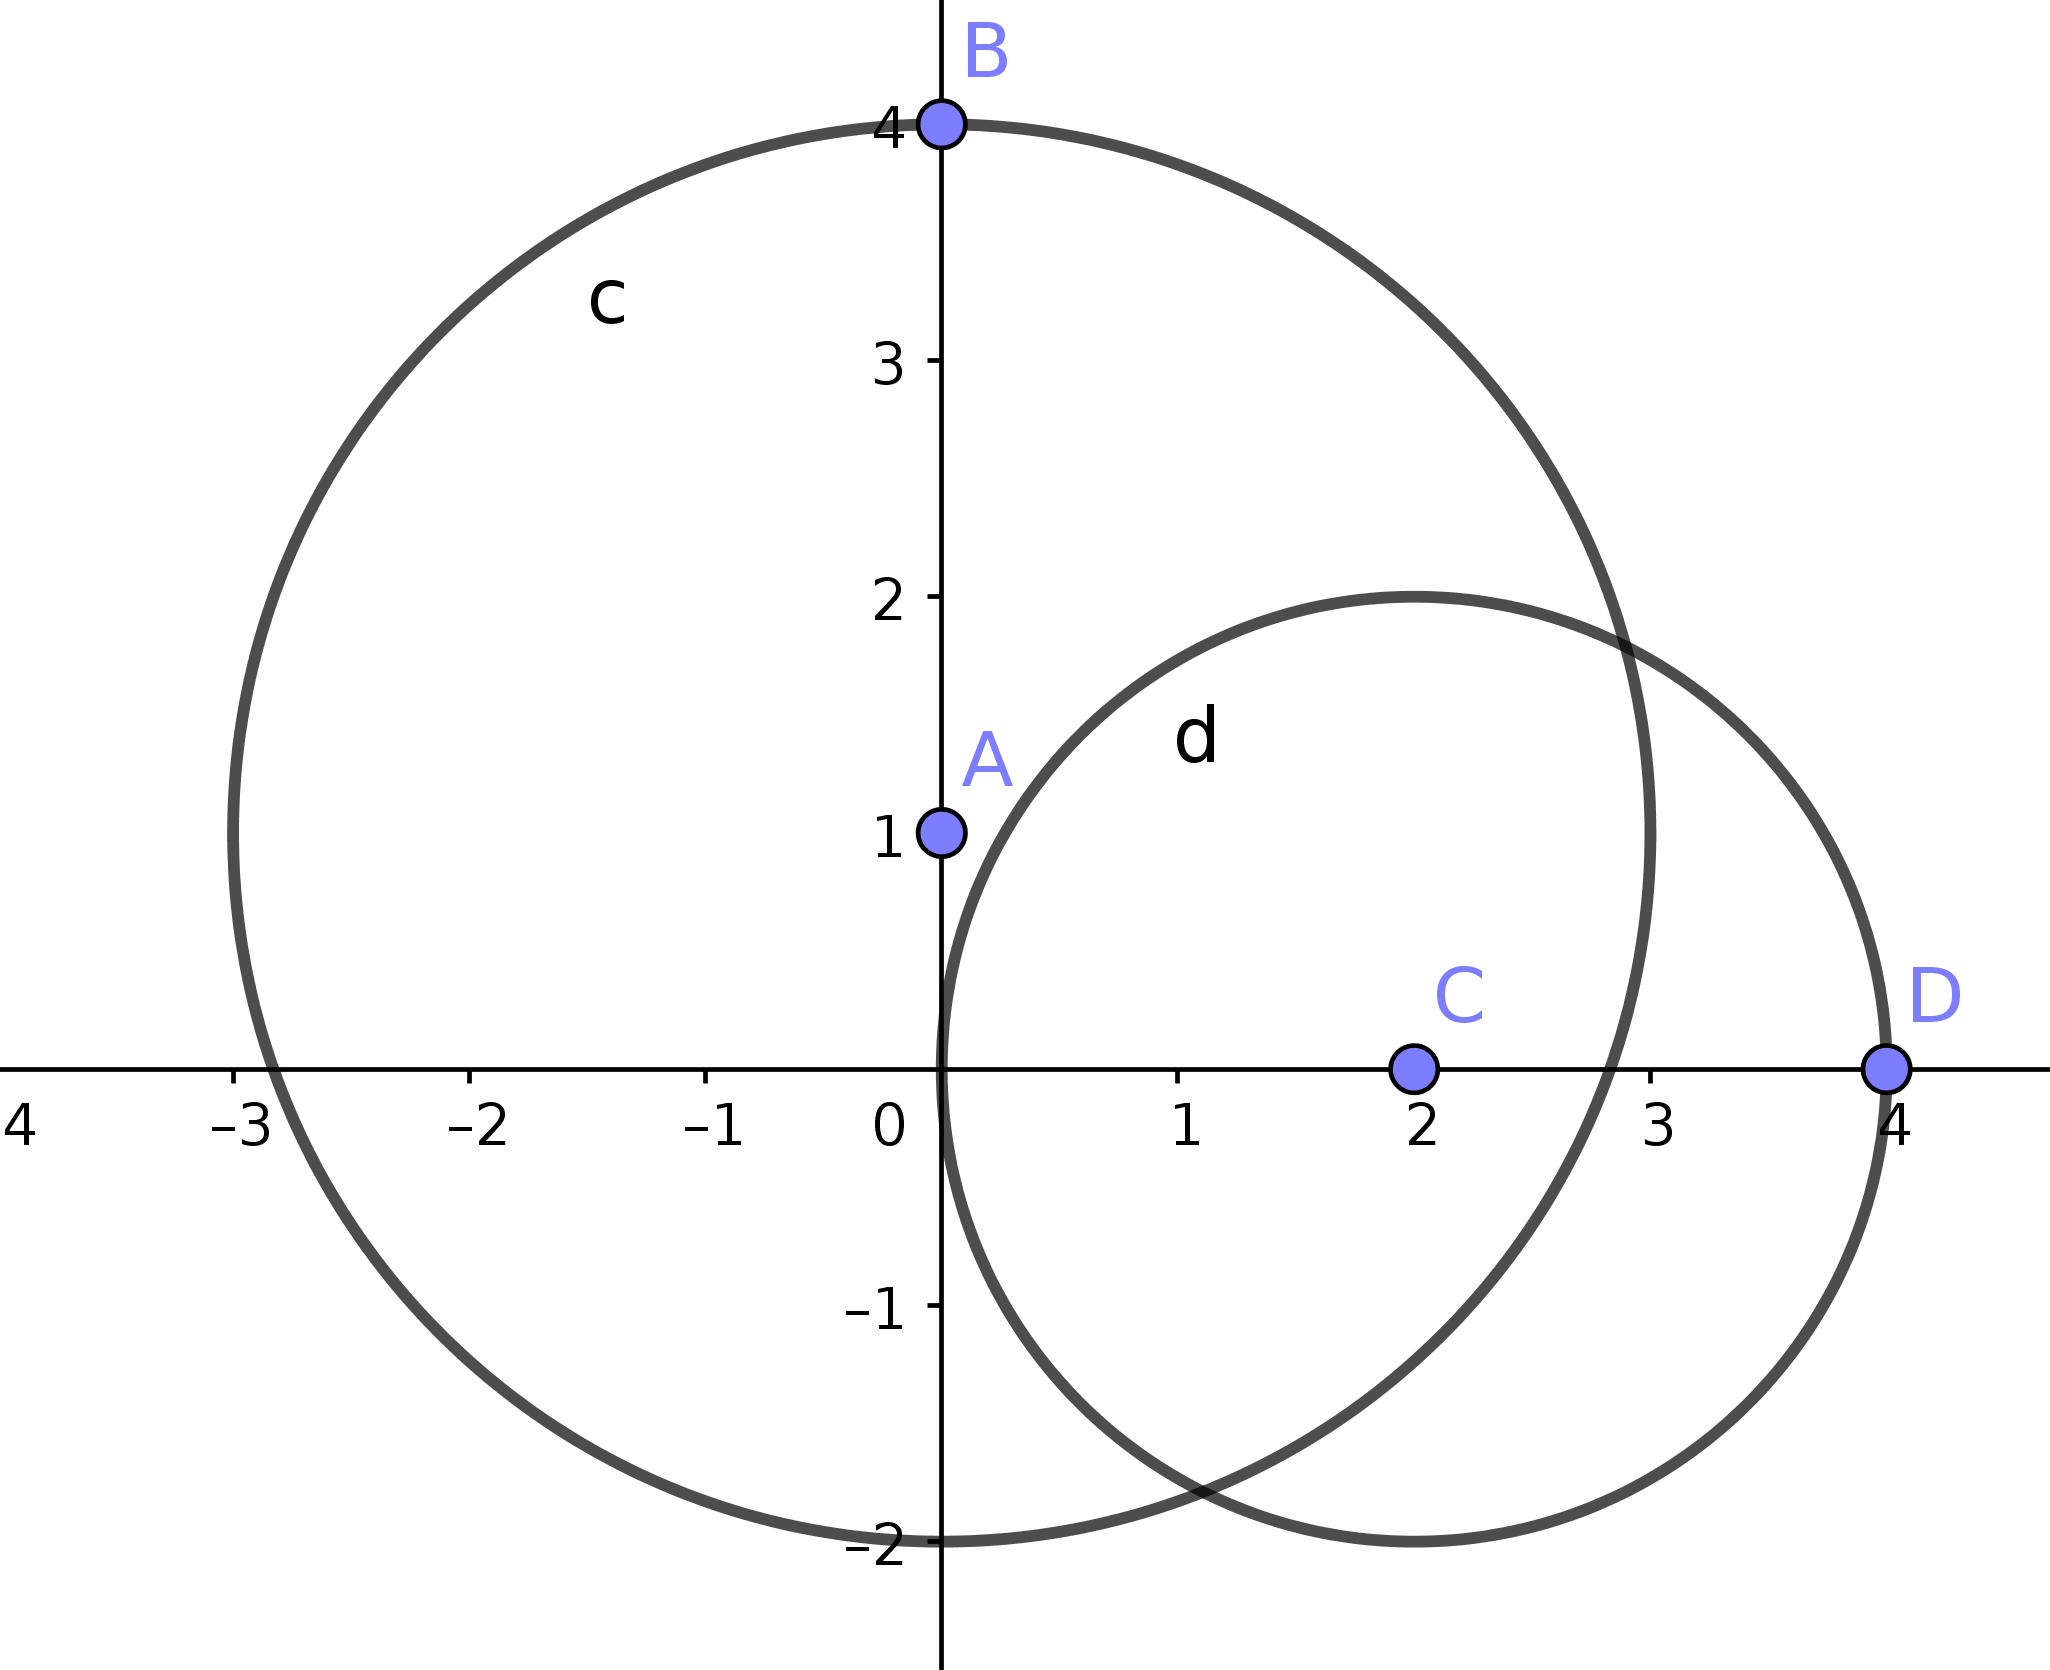
\includegraphics[height=0.2\textheight]{circs}
	 \caption{Posição das circunferências.}\label{circs}
	 \end{figure}
	\end{ans}
	




%%%%%%%%%% 4
\item Considere a reta $r$ no plano dada pela equação geral $2x-y=3$. Analise as alternativas e assinale a correta.
	\begin{enumerate}
	\F\alt A reta $s$ de equação $2x+y=3$ é perpendicular à reta $r$.
	\V\alt A reta $s$ de equação $4x-2y=-7$ é paralela à reta $r$.
	\F\alt A origem do sistema, ponto $(0,0)$, pertence à reta $r$.
	\V\alt A reta $s$ de equação $x+2y=7$ é perpendicular à reta $r$.
	\V\alt A reta $s$ de equação $-x+2y=3$ é paralela à reta $r$.
	\end{enumerate}
	
	\begin{ans}
	Precisamos dos vetores diretores de cada uma das retas. Vou fazer apenas um deles, os demais são análogos.
	
	Tome a reta $2x-y=3$. Isole uma das variáveis, digamos, $y$. Com isso, temos $y=2x-3$. Agora, vamos parametrizar $x$ e $y$, fazendo-os $x(t)$ e $y(t)$. A variável dependente $y$ continuará dependente, e a variável independente $x$ será idêntica ao parâmetro $t$.
	\[
	\begin{cases}
	x(t)=t\\
	y(t)=2t-3
	\end{cases}
	\]
	Perceba que esse sistema de equações é o mesmo que $X=(x,y)=(1,2)t+(0,-3)$, conforme já vimos. E o vetor diretor é, portanto, $(1,2)$.
	
	Para saber se duas retas são paralelas, basta verificar se seus vetores diretores (vd) são proporcionais, isto é, exista $k$ de modo que $k \cdot vd(r)=vd(s)$. Para verificar se são perpendiculares, basta que o produto interno de seus vetores diretores seja zero $\langle vd(r),vd(s) \rangle =0$. Para saber se um ponto pertence à reta, basta substituí-lo na equação e verificar a igualdade.
	
	(a) vetor diretor $(1,-2)$, cujo produto interno com o vd da reta dada \textbf{não} é zero.\\
	(b) vetor diretor $(1,2)$ é proporcional ao vd da reta dada.\\
	(c) o ponto $(0,0)$ \textbf{não} satisfaz a equação da reta dada.\\
	(d) vetor diretor $(-2,1)$, cujo produto interno com o vd da reta dada é zero.\\
	(e) vetor diretor $(2,1)$ \textbf{não} é proporcional ao vd da reta dada.
	\end{ans}





%%%%%%%%%% 5
\item A área de uma elipse na forma reduzida $\tfrac{x^2}{a^2}+\tfrac{y^2}{b^2}=1$ pode ser calculada através da expressão $\text{área}=\pi ab$. Qual é a área da elipse $\tfrac{x^2}{27}+\tfrac{y^2}{12}=1$?
	
	\begin{enumerate}
	\alt $324\pi$ unidades de área.
	\alt $36\pi$ unidades de área.
	\X\alt $18\pi$ unidades de área.
	\alt $12\pi$ unidades de área.
	\alt $6\sqrt{3}\pi$ unidades de área.
	\end{enumerate}
	
	\begin{ans}
	A resposta é bem simples, basta fazer contas: $\tfrac{x^2}{27}+\tfrac{y^2}{12}=1$ significa que $a^2=27=3 \cdot 3^2$ e $b^2=12=3\cdot 2^2$, ou seja, $a=3\sqrt{3}$ e $b=2\sqrt{3}$. Assim,  $\text{área}=\pi3\cdot2\sqrt{3}\sqrt{3}=18\pi$.
	\end{ans}








%%%%%%%%%% 6
\item Qual é o perímetro do triângulo em que os vértices são os pontos médios dos segmentos $\overline{AB}$, $\overline{BC}$ e $\overline{AC}$? Sabendo-se que as coordenadas dos pontos são $A=(0,0)$, $B=(3,4)$ e $C=(-3,4)$. Todas as medidas estão em metros.
	\begin{enumerate}
	\X\alt $8m$. 
	\alt $12m$.
	\alt $16m$.
	\alt $6\sqrt{2}m$.
	\alt $8\sqrt{2}m$.
	\end{enumerate}
	
	
	\begin{ans}
	Em geometria analítica, um ponto X que \emph{dista igualmente} de um conjunto de pontos \{A,B,C,D\}, por exemplo, é simplesmente a média aritmética entre eles, ou seja, $X=(A+B+C+D)/4$. Assim, o ponto médio entre dois pontos é a média aritmética entre eles: 
\[
\begin{aligned}
R=M_{AB}&=(A+B)/2=\big((0,0)+(3,4)\big)/2=(3/2,2);\\
S=M_{BC}&=(B+C)/2=\big((3,4)+(-3,4)\big)/2=(0,4);\\
T=M_{AC}&=(A+C)/2=\big((0,0)+(-3,4)\big)/2=(-3/2,2).
\end{aligned}
\]
	Agora que temos os vértices do triângulo, precisamos calcular as medidas dos lados. Fazemos isso calculando os módulos de vetores, como segue:
\[
	\begin{aligned}
		\overrightarrow{RS} = S-R &= (0,4)-(3/2,2) = (-3/2,2)\\
		\overrightarrow{ST} = T-S &= (-3/2,2) - (0,4) = (-3/2,-2)\\
		\overrightarrow{RT} = T-R &= (-3/2,2) - (3/2,2) = (-3,0)
	\end{aligned}
\]
\[
	\begin{aligned}
		\left|\overrightarrow{RS}\right| &= \sqrt{(-3/2)^2+2^2}=\sqrt{25/4}=5/2\\
		\left|\overrightarrow{ST}\right| &= \sqrt{(-3/2)^2+(-2)^2}=\sqrt{25/4}=5/2\\
		\left|\overrightarrow{RT}\right| &= \sqrt{(-3)^2+0^2}=\sqrt{9}=3
	\end{aligned}
\]
	Essas são as medidas dos lados do triângulo, e portanto seu perímetro é $5/2+5/2+3=8$.
	\end{ans}









%%%%%%%%%% 7
\item Seja $\vec u$ um vetor não nulo. A projeção ortogonal de um vetor $\vec v$ qualquer sobre o vetor $\vec u$ é dada pela expressão
	\[
	\proj_{\vec u} \vec v = \dfrac{(\vec u,\vec v)}{|\vec u|^2}\vec u,
	\]
	onde $(\vec u,\vec v)$ significa o produto interno dos vetores $\vec u$ e $\vec v$; $|\vec u|$ é o módulo do vetor $\vec u$. Lembre-se que o módulo de um vetor qualquer $X=(a,b,c)$ é dado por $|X|=\sqrt{a^2+b^2+c^2}\color{Cyan}=\!\sqrt{\sum_i X_i^2}$. Por exemplo, o módulo do vetor $X=(1,1,2)$ é $|X|=\sqrt{1^2+ 1^2 +2^2}=\sqrt{6}$. Diante do exposto, qual é o módulo da projeção ortogonal do vetor $(2,4,1)$ sobre o vetor $(4,2,-4)$?
	\begin{enumerate}
	\X\alt $2$.
	\alt $4$.
	\alt $\frac{4}{\sqrt{21}}$.
	\alt $\frac{8}{\sqrt{21}}$.
	\alt $8$.
	\end{enumerate}
	
	\begin{ans}
	Temos dois escalares para calcular: o produto interno $(\vec u,\vec v)=\sum_i \vec u_i\vec v_i$ e o módulo de $\vec u$ ao quadrado $|\vec u|^2=\left(\sqrt{\sum_i \vec u_i^2}\right)^2=\sum_i \vec u_i^2$. Então $(\vec u,\vec v)=2\cdot 4+4\cdot 2+1\cdot(-4)=12$. Temos também $|\vec u|^2=|(4,2,-4)|^2=4^2+2^2+(-4)^2=16+4+16=36$.
	Portanto
	\[
	\proj_{\vec u}\vec v=\frac{12}{36}\vec u=\frac{1}{3}(4,2,-4).
	\]
	Agora, falta calcular o módulo desse vetor:
	\[
	|\;\proj_{\vec u}\vec v\;| = \frac{1}{3}\sqrt{\left(4^2+2^2+(-4)^2\right)} = \frac{1}{3}\sqrt{36}=\frac{6}{3}=2.
	\]
	\end{ans}



%%%%%%%%%% 8
\item Considere os planos $\pi_1:x-y+4z=-4$ e $\pi_2:2x+y-z=7$ e o ponto $P=(1,1,0)$. Calcule a distância entre a reta $r$ e o ponto $P$, sabendo que a reta $r$ é a interseção dos planos $\pi_1$ e $\pi_2$.

Sugestão: utilize a fórmula de distância de ponto e reta $d(P,r)=\frac{|\vec v\times\overrightarrow{AP}|}{|\vec v|}$, onde $\vec v\times\overrightarrow{AP}$ é o produto vetorial entre o vetor diretor da reta $\vec v$ e o vetor $\overrightarrow{AP}$, em que $A$ é um ponto qualquer da reta.
	\begin{enumerate}
	\alt $\frac{4}{\sqrt{21}}$.
	\alt $\frac{4}{\sqrt{11}}$.
	\X\alt $\frac{4\sqrt{2}}{\sqrt{11}}$.
	\alt $\frac{4\sqrt{2}}{\sqrt{21}}$.
	\alt $4$.
	\end{enumerate}
	
	\begin{ans}
	Para calcular a reta que é interseção entre os planos, vamos precisar de dois pontos $R$ e $S$ que satisfaçam a ambas as equações dos planos (dois pontos determinam uma reta). Para o ponto $R$ vamos fixar a abscissa $x=0$, e para o ponto $S$ vamos fixar a cota $z=0$. Agora, calculamos as demais coordenadas de $R$ e $S$. 
	
	\[
	R=(0,y,z) \qquad S=(x,y,0)
	\]
	\[
	(\pi_1\cap\pi_2)(R)=
	\begin{cases}
		-y+4z=-4\\
		y-z=7	
	\end{cases}
	\qquad
	(\pi_1\cap\pi_2)(S)=
	\begin{cases}
		x-y=-4\\
		2x+y=7	
	\end{cases}
	\]
	Resolvendo esses sistemas lineares obtemos $R=(0,8,1)$ e $S=(1,5,0)$.
	Um vetor diretor da reta é o vetor $\overrightarrow{RS}=S-R=(1,-3,-1)$. Um ponto por onde essa reta passa pode ser, por exemplo, $R$ ou mesmo $S$. Tomemos $R$. A equação da reta que é interseção entre os planos é então
	\[
		r=(\pi_1\cap\pi_2):\quad X=(1,-3,-1)t+(0,8,1).
	\]
	Façamos $A=R$. Calcularemos o produto vetorial entre o vd da reta $\vec v=(1,-3,-1)$ e o vetor $\overrightarrow{AP}=P-A=(1,1,0)-(0,8,1)=(1,-7,-1)$.
	\[
	\vec v\times \overrightarrow{AP}=
	\det
	\begin{vmatrix}
	i & j & k\\
	1 & -3 & -1\\
	1 & -7 & -1
	\end{vmatrix}
	=3i-7i-j+j-7k+3k=(-4,0,-4)
	\]
	Por fim, calculamos a razão entre os módulos dos vetores $\vec v\times \overrightarrow{AP}$ e $\vec v$ para obter a resposta:
	\[
	d(P,r)=\frac{|\vec v\times\overrightarrow{AP}|}{|\vec v|}=\frac{|\sqrt{(-4)^2+0^2+(-4)^2}|}{|\sqrt{1^2+(-3)^2+(-1)^2}|}=\frac{4\sqrt{2}}{\sqrt{11}}.
	\]
	\end{ans}
	




%%%%%%%%%% 9
\item Considere as elipses $E_1$ e $E_2$ de equações $E_1: \frac{x^2}{25}+\frac{y^2}{16}=1$ e $E_1: \frac{x^2}{169}+\frac{y^2}{4}=1$. Analise as sentenças e assinale a alternativa correta.

	\begin{enumerate}[label=\Roman*.]
	\V\alt A elipse $E_2$ é mais achatada que a elipse $E_1$.
	\V\alt Os focos da elipse $E_1$ estão no eixo $x$.
	\V\alt O tamanho do eixo maior da elipse $E_1$ é igual a $10$.
	\end{enumerate}
	
	\begin{enumerate}
	\alt Apenas a sentença I está correta.
	\alt As sentenças I e II estão corretas.
	\alt As sentenças I e III estão corretas.
	\alt As sentenças II e III estão corretas.
	\X\alt As sentenças I, II e III estão corretas.
	\end{enumerate}
	
	\begin{ans}
	Para responder a I, II e III, basta analisar o que acontece com as equações, quando $x=0$ ou quando $y=0$.
		\begin{description}
		\item[se $x=0$ (sobre o eixo y):] \ 
			\begin{itemize}
			\item $E_1:\frac{y^2}{16}=1$ significa que $y=\pm 4$, isto é, a interseção de $E_1$ com o eixo $y$ se dá nos pontos $(0,-4)$ e $(0,4)$.
			\item $E_2:\frac{y^2}{4}=1$ significa que $y=\pm 2$, isto é, a interseção de $E_2$ com o eixo $y$ se dá nos pontos $(0,-2)$ e $(0,2)$.
			\end{itemize}
		\item[se $y=0$ (sobre o eixo x):] \ 
		\begin{itemize}
			\item $E_1:\frac{x^2}{25}=1$ significa que $x=\pm 5$, isto é, a interseção de $E_1$ com o eixo $x$ se dá nos pontos $(-5,0)$ e $(5,0)$.
			\item $E_2:\frac{x^2}{169}=1$ significa que $x=\pm 13$, isto é, a interseção de $E_2$ com o eixo $x$ se dá nos pontos $(-13,0)$ e $(13,0)$.
			\end{itemize}
		\end{description}
		Esses são os 4 vértices de ambas as elipses. Com esses pontos, podemos fazer o esboço das elipses. O esboço delas consta na Figura \ref{elipses}. 
		
		\begin{figure}[H]\centering
		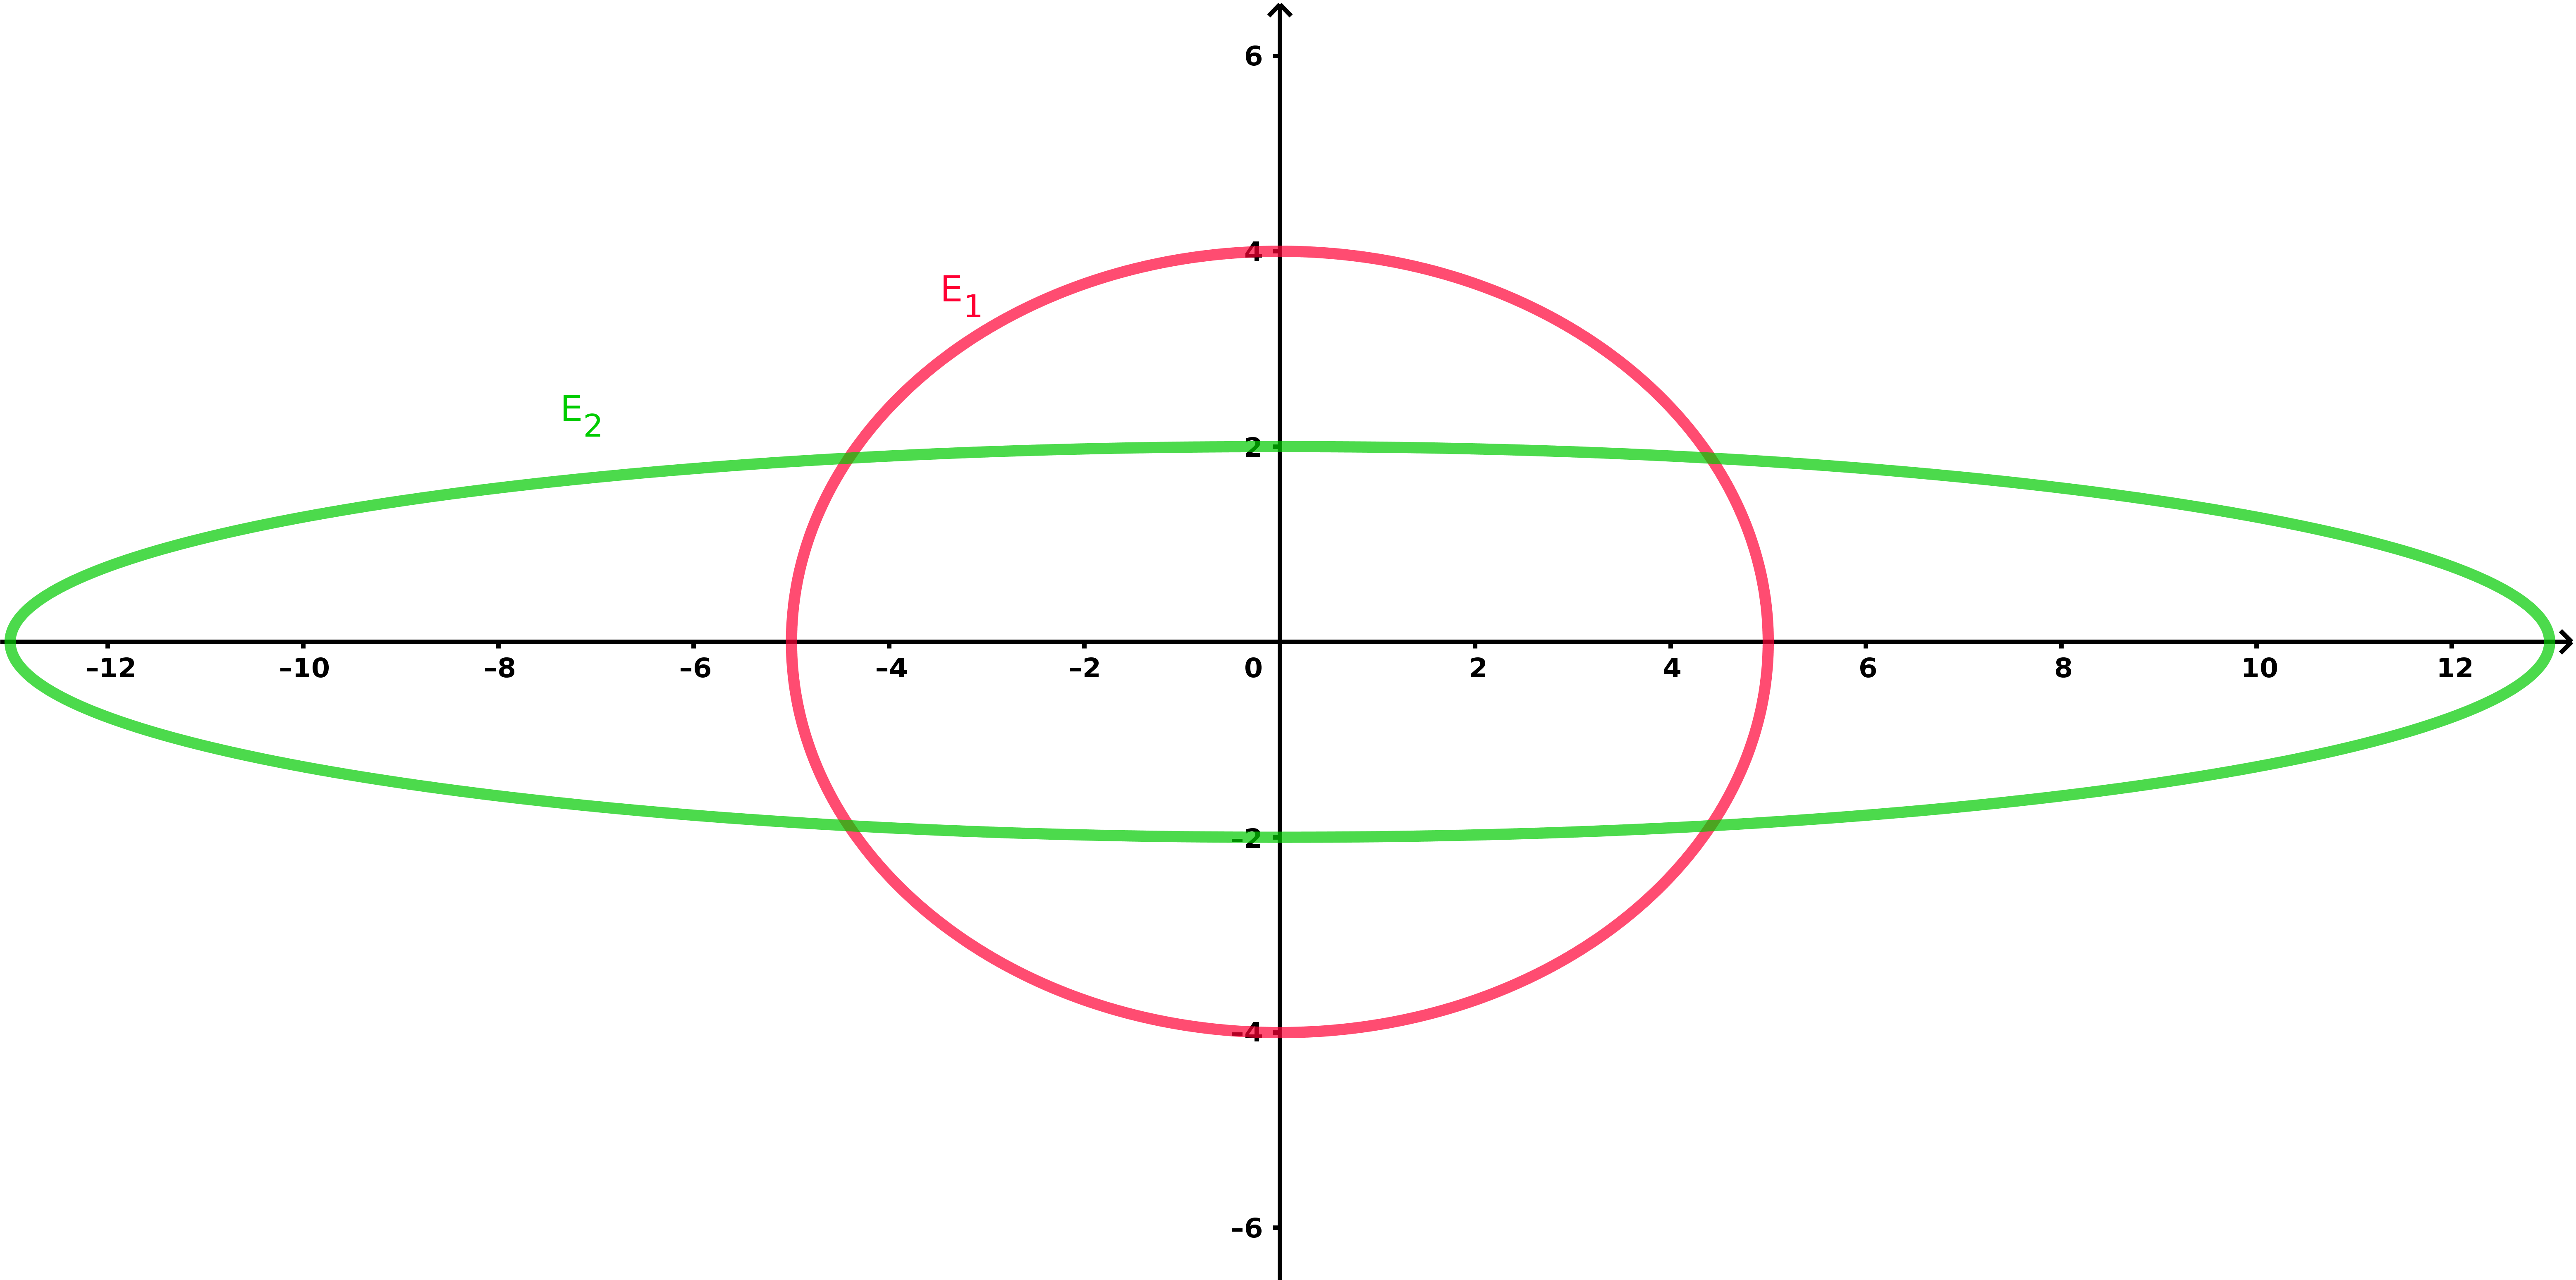
\includegraphics[width=0.8\textwidth]{fig}
		\caption{Elipses}\label{elipses}
		\end{figure}
	
	\end{ans}
	

%%%%%%%%%% 10	
\item Qual é a equação da hipérbole de centro na origem, focos nos pontos $F_1=(-4,0)$ e $F_2=(4,0)$ e a medida do eixo real (ou transverso)	igual a $6$? 
	\begin{enumerate}
	\F\alt $\frac{x^2}{5}-\frac{y^2}{9}=1$.
	\F\alt $\frac{x^2}{9}-\frac{y^2}{5}=1$.
	\F\alt $\frac{x^2}{9}-\frac{y^2}{25}=1$.
	\F\alt $\frac{y^2}{5}-\frac{x^2}{9}=1$.
	\F\alt $\frac{x^2}{25}-\frac{y^2}{9}=1$.
	\end{enumerate}
	
	\begin{ans}
	A distância entre os focos, ou distância focal, é definida como $2c$, e a distância entre os vértices da hipérbole é definida como $2a$ (eixo transverso). O eixo conjugado ou imaginário tem comprimento definido como $2b$, em que $a^2+b^2=c^2$. Assim, podemos calcular $a$, $b$ e $c$ a partir dos dados do problema.
	\[
	2c = |F_1-F_2|=|(-4,0)-(4,0)|=8 \iff c=4;
	\]
	\[
	2a = 6 \iff a = 3;
	\]
	\[
	b^2 = c^2-a^2 \iff b^2 = 16-9=7.
	\]
	A equação de uma hipérbole \textbf{cujo eixo transverso está sobre o eixo $x$} é dada por 
	\[
	\frac{x^2}{a^2}-\frac{y^2}{b^2}=1.
	\]
	Assim, a equação da hipérbole desejada é
	\[
	\frac{x^2}{9}-\frac{y^2}{7}=1.
	\]
	\end{ans}
	
	
\end{enumerate}

\end{document}